\documentclass[11pt]{article}
\usepackage{amssymb,amsmath,amsthm}
\usepackage{bm, mathrsfs}
\usepackage{graphicx}
\usepackage{geometry}
\usepackage{textcomp}
\usepackage{hyperref}
\usepackage{ragged2e}
\usepackage{float}
\graphicspath{ {./images/} }
\newtheorem{remark}{Remarque}
\newcommand{\bx}{\bm{x}}

\title{ISC3, Fall 2022 (A22) \\
 Computer works report TP 3, 03/10/2022}
\author{Wenlong CHEN}
\date{October 8, 2022}

\begin{document}
    \maketitle
    \section*{Exercise 1}
    Let $(x,y,z) \rightarrow F(x,y,z)$ be the mapping defined by
    $$
    F(x,y,z)=
    \begin{bmatrix}
        (x-2)^2-1 \\
        (y-z-3)^2 \\
        (z+1)^2-1
    \end{bmatrix}
    $$
    Write a Scilab function Fout=F(xvec) that implements the mapping \textbf{F}, and a Scilab function Jout=FJac(xvec) that computes the Jacobian matrix of \textbf{F}.\\
    ~\\
    Solution : \\
    Sur la base de la définition de la matrice de Jacobi et de la fonction F, nous pouvons écrire la matrice de Jacobi de la fonction F
    $$
    \begin{bmatrix}
        2*(x-2) & 0 & 0 \\
        0 & 2*(y-z-3) & -2*(y-z-3) \\
        0 & 0 & 2*(z+1)
    \end{bmatrix}
    $$
    Code pour cette question : 
    \begin{verbatim}
        function Fout = F(xvec)
            Fout = zeros(1,3)
            Fout(1) = (xvec(1) - 2)^2 - 1
            Fout(2) = (xvec(2) - xvec(3) - 3)^2
            Fout(3) = (xvec(3) + 1)^2 - 1
        endfunction

        function Jout = FJac(xvec)
            Jout = zeros(3,3)
            Jout(1,1) = 2 * (xvec(1) - 2)
            Jout(2,2) = 2 * (xvec(2) - xvec(3) - 3)
            Jout(2,3) = -2 * (xvec(2) - xvec(3) - 3)
            Jout(3,3) = 2 * (xvec(3) + 1)
        endfunction
    \end{verbatim}
    ~\\

    \section*{Exercise 2}
    Implement the Newton method that numerically solve $F(x) = 0$. Use $x_0 =(0,0,0)$ as initial guess.\\
    ~\\
    Solution : \\
    Pour une erreur de $10^{-5}$, seules onze itérations sont utilisées pour obtenir $x=(1,3,0)$.\\
    ~\\
    Code pour cette question :
    \begin{verbatim}
        function [x,k]=Newton(x0,Fout,Jout,err) // k est le Nombre d'itérations
            k=1;x=x0;
            while abs(norm(F(x))) >err
                x = x+(-Jout(x)\Fout(x)')
                k=k+1
            end
        endfunction

        [x,k] = Newton(zeros(3,1),F,FJac,10^(-5))
    \end{verbatim}
    ~\\

    \section*{Exercise 3}
    Consider an articulated arm made of two rods of respective length 4 and 3. The articulated arm is fixed at the origin $O(0,0)$. The midpoint $A$ that binds the two rods has coordinates $A(x,y)$. The free endpoint is denoted by $B$.\\
    ~\\
    (a) Find $(x,y)$ such that B = $(3,3)$.\\
    Solution :\\
    D'après les fonctions trigonométriques, on peut savoir que :
    $$
    \begin{matrix}
        x^2+y^2=4^2 \\
        (x-3)^2+(y-3)^2=3^2
    \end{matrix}
    $$
    A la fin, on peut obtenir $A=(0.1703,3.9964)$\\
    Code pour cette question :
    \begin{verbatim}
        function E3_1=F3_1(xvec)
            E3_1(1) = xvec(1)^2 + xvec(2)^2 - 16
            E3_1(2) = (xvec(1) - 3)^2 + (xvec(2) - 3)^2 - 9
        endfunction

        xE3_1 = fsolve(zeros(2,1),F3_1)
    \end{verbatim}
    (b) Find the two angles $\theta_1$ and $\theta_2$ made by the two rods with the horizontal axis. Use the Scilab fsolve() function to answer the 2 questions.\\
    ~\\
    Solution :
    D'après les fonctions trigonométriques, on peut savoir que :
    $$
    \begin{matrix}
        sin(\theta_1) = \frac{y}{4}\\
        sin(\theta_2) = \frac{y-3}{3}
    \end{matrix}
    $$
    Code pour cette question :
    \begin{verbatim}
        function E3_2 = F3_2(theta)
            E3_2(1) = sin(theta(1)) - xE3_1(2)/4
            E3_2(2) = sin(theta(2)) - (xE3_1(2)-3)/3
        endfunction
        xE3_2 = fsolve(zeros(2,1),F3_2)
        xE3_2 = xE3_2/%pi .* 180
    \end{verbatim}


    \section*{Exercise 4}
    Draw a perfect pentagon by solving an algebraic system of equations $F(x) = 0$\\
    ~\\
    Solution :
    La somme des angles intérieurs du pentagone est de 540 degrés et les cinq angles intérieurs sont de 72 degrés. La conversion des coordonnées d'entrée en coordonnées polaires permet de résoudre facilement le problème.\\
    Convertir d'abord les coordonnées cartésiennes en coordonnées polaires:
    $$
    \begin{matrix}
        \rho_0=\sqrt{x_0^2+y_0^2}\\
        \theta_0=atan2(y,x)
    \end{matrix}
    $$
    Le système d'équations suivant peut être dérivé du titre:
    $$
    \begin{matrix}
        \rho=\rho_0\\
        \theta=\theta_0+\frac{72*\pi}{180}
    \end{matrix}
    $$
    Après avoir résolu le système d'équations, convertissez les coordonnées polaires en coordonnées cartésiennes:
    $$
    \begin{matrix}
        x=\rho*sin(\theta)\\
        y=\rho*cos(\theta)
    \end{matrix}
    $$
    Soit un point du pentagone (0,1), la résolution de l'équation vous donnera les coordonnées des quatre autres points et finalement vous pourrez dessiner le diagramme ci-dessous
    \begin{figure}[H]
        \centering
        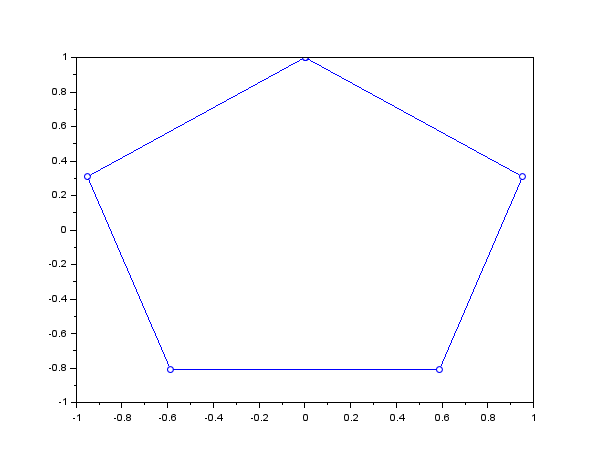
\includegraphics[width=0.8\textwidth,height=0.5\textwidth]{pen}
        \caption{L'image du pentagone}
    \end{figure}
    Code pour cette question :
    \begin{verbatim}
        x=0;y=1
        function E4=F4(xvec)
            p=sqrt(y^2+x^2)
            if x>0 then
                theta=atan(y/x)
            end
            if x<0&&y>=0 then
                theta=atan(y/x)+%pi
            end
            if x<0&&y<0 then
                theta=atan(y/x)-%pi
            end
            if x==0&&y>0 then
                theta=%pi/2
            end
            if x==0&&y<0 then
                theta=-%pi/2
            end
            E4(2) = xvec(2) - theta-72/180*%pi
            E4(1) = xvec(1) - p
        endfunction

        E4(:,1)=[1;atan(y/x)]
        for i=1:5
            E4(:,i+1)=fsolve([0;0],F4)
            x=E4(1,i+1)*cos(E4(2,i+1))
            y=E4(1,i+1)*sin(E4(2,i+1))
        end
        plot( (E4(1,:).*cos(E4(2,:))) ,(E4(1,:).*sin(E4(2,:))))
    \end{verbatim}

    \section*{Exercise 5}
    The objective of this exercise is to determine the intersection(s) of the 3D sphere of center $O$ and radius 1, the sphere of center $(1,0,0)$ and radius 1 and the plane of equation $x + y +z = 0$. Write the system of equations to solve, write the corresponding function $F(x)$, compute its Jacobian matrix, and apply the Scilab function fsolve() with the F function and its Jacobian as entry arguments.\\
    ~\\
    Solution :
    $$
    F=
    \begin{bmatrix}
        x^2+y^2+z^2=1\\
        (x-1)^2+y^2+z^2=1\\
        x+y+1=0
    \end{bmatrix}
    ,
    J=
    \begin{bmatrix}
        2*x & 2*y & 2*z\\
        2*(x-1) & 2*y & 2*z\\
        1 & 1 & 1
    \end{bmatrix}
    $$
    Selon l'image de la fonction, il devrait y avoir deux points d'intersection, mais fsovle() ne peut trouver qu'une seule solution, nous devons changer la valeur initiale de fsovle() pour trouver deux solutions\\
    Selon le calcul, nous pouvons obtenir intersections=$(0.5,0.309,-0.809),(0.5,-0.809,0.309)$. 
    ~\\
    Cdoe pour cette question :
    \begin{verbatim}
        function E5=F5(xvec)
            E5(1) = xvec(1)^2 + xvec(2)^2 + xvec(3)^2 -1
            E5(2) = (xvec(1)-1)^2 + xvec(2)^2 + xvec(3)^2 - 1
            E5(3) =  xvec(1) +  xvec(2) + xvec(3)
        endfunction
        function J=FJ(xvec)
            J(1,1) = 2*xvec(1)
            J(1,2) = 2*xvec(2)
            J(1,3) = 2*xvec(3)
            J(2,1) = 2*(xvec(1)-1)
            J(2,2) = 2*xvec(2)
            J(2,3) = 2*xvec(3)
            J(3,1) = 1
            J(3,2) = 1
            J(3,3) = 1
        endfunction

        xE5=fsolve([5;5;5],F5,FJ)
        xE5_2=fsolve([5;-5;5],F5,FJ)
    \end{verbatim}
    \section*{Résumé}
    Nous devons faire attention au nombre de solutions lorsque nous utilisons fsolve(), car il utilise la valeur initiale pour calculer le zéro le plus proche
    En même temps, nous devons veiller à transformer le problème en une forme plus simple lorsque nous le résolvons.
    Par exemple, à la question 4, dessiner le pentagone en utilisant un système de coordonnées normales à angle droit serait fastidieux, alors que l'utilisation d'un système de coordonnées polaires le simplifierait considérablement.
\end{document}